\documentclass[conference]{IEEEtran}
\IEEEoverridecommandlockouts
% The preceding line is only needed to identify funding in the first footnote. If that is unneeded, please comment it out.
\usepackage{cite}
\usepackage{amsmath,amssymb,amsfonts}
\usepackage{algorithmic}
\usepackage{graphicx}
\usepackage{textcomp}
\usepackage{xcolor}
\def\BibTeX{{\rm B\kern-.05em{\sc i\kern-.025em b}\kern-.08em
    T\kern-.1667em\lower.7ex\hbox{E}\kern-.125emX}}
\renewcommand\IEEEkeywordsname{Keywords}

\begin{document}

\title{ Implementation of Grover’s Algorithm based on
	Quantum Reservoir Computing  \\

}
\author{\IEEEauthorblockN{Shivani Mehta}
	\IEEEauthorblockA{\textit{Department of ECE,} \\
		\textit{IIITDM Kancheepuram,}\\
		Chennai-600127, India.\\
		ec22m2002@iiitdm.ac.in}
	\and
	\IEEEauthorblockN{Sajja Jyothikrishna}
	\IEEEauthorblockA{\textit{Department of ECE,} \\
		\textit{IIITDM Kancheepuram,}\\
		Chennai-600127, India. \\
		ec21b1022@iiitdm.ac.in}
	\and
	\IEEEauthorblockN{V.Praveen Bhallamudi}
	\IEEEauthorblockA{\textit{Department of Physics,} \\
		\textit{IIITDM Kancheepuram,}\\
		Chennai-600036, India. \\
		praveen.bhallamudi@iitm.ac.in}
	\and
	\IEEEauthorblockN{Sumanth Arige}
	\IEEEauthorblockA{\textit{Department of ECE,} \\
		\textit{IIITDM Kancheepuram,}\\
		Chennai-600127, India. \\
		edm20d010@iiitdm.ac.in}
	\and

	\IEEEauthorblockN{ Tejendra Dixit, $Member, IEEE$}
	\IEEEauthorblockA{\textit{Department of ECE,} \\
		\textit{IIITDM Kancheepuram,}\\
		Chennai-600127, India. \\
		tdixit@iiitdm.ac.in}
}

\maketitle

\begin{abstract}
	Quantum computing represents the leading edge of
	computational technology, leveraging the principles of quantum
	mechanics to execute targeted computations much faster than
	classical computers. In contrast to classical bits, which are limited
	to representing either 0 or 1, qubits, or quantum bits, exhibit
	the extraordinary property of superposition. This distinctive
	characteristic enables qubits to simultaneously occupy multiple
	states, empowering quantum computers to explore numerous
	potential solutions to a problem concurrently. This feature
	makes quantum computing particularly potent for specific tasks.
	Recent research endeavors have been sparked by the potential
	of advanced quantum computing technology, leading to the
	creation of simulations of quantum computers using classical
	hardware. Grover’s quantum search algorithm serves as a notable
	illustration of quantum computing application, enabling quantum
	computers to conduct a database search within an unsorted array
	with a quadratic speedup in time efficiency compared to classical
	computers. This document presents the quantum Grover search
	algorithm and its application through 5-qubit quantum circuits,
	as well as a design framework to simplify the creation of an
	oracle for a greater number of qubits.
\end{abstract}

\begin{IEEEkeywords}
	Quantum computation, Qubits, Oracle, Grover’s
	algorithm, IBM Qiskit.
\end{IEEEkeywords}

\section{Introduction}
The exploration of quantum computing [1][2] falls within
the realm of quantum information science, which revolves
around the fundamental principles of storing and manipulating
information. In this work, we delved into quantum computing,
acquiring a comprehensive understanding of quantum bits
and their properties, as well as leveraging these properties
to tackle problems. We familiarized ourselves with quantum
gates and their operations on qubits, simulating all the funda
mental quantum gates [3][4]. Additionally, we delved into the
Grover search algorithm and implemented quantum gates for
Grover operations. Quantum computers exhibit significantly
faster speeds compared to classical computers [5][6]. In the
case of an unsorted dataset with size N, classical computers
usually demand O(N) operations, whereas Grover’s algorithm
accomplishes this task optimally in O($\sqrt{N}$) operations.
\\
We
executed the algorithm using Qiskit, an IBM tool for com
puting quantum circuits, and conducted simulations for the
Grover algorithm [7], presenting the results graphically with
the probability of obtaining the correct output.

Within Grover’s quantum search algorithm, a network with
n qubits harbors $ 2^{n} $ = N states, with each state bearing a
probability of $ 1/N $ for discovery. Consequently, the amplitude
of each state is $ 1/\sqrt{N} $
. Conversely, classical systems tackling the
same problem necessitate a maximum of O(N) trials.
\section{Background and Methodology}

The Grover search algorithm, conceived by Lov Grover
in 1996, stands as a quantum computing method offering
a quadratic acceleration compared to classical counterparts,
particularly for solving unstructured search problems [8]. It
has gained renown for its proficiency in searching through
unsorted databases, but its utility extends to a spectrum
of tasks, encompassing cryptographic problem-solving and
quantum system simulation. This can speed up a search
problem quadratically. For N number of unsorted data classical
computer require O (N) operations Whereas Grover is optimal
and can do this in O($ \sqrt{N} $) operation. The following provides
a synopsis of the workings of the Grover search algorithm [9]:
\subsection{Initialisation}
Commencing the process involves establishing a superposition of all conceivable states. For instance, when seeking an
item in a database housing N item, quantum parallelism is
harnessed to generate a superposition of all N states as shown
in Fig.1. Achieving this involves a sequence of quantum gate
operations.

\begin{figure}[htbp]
	\centerline{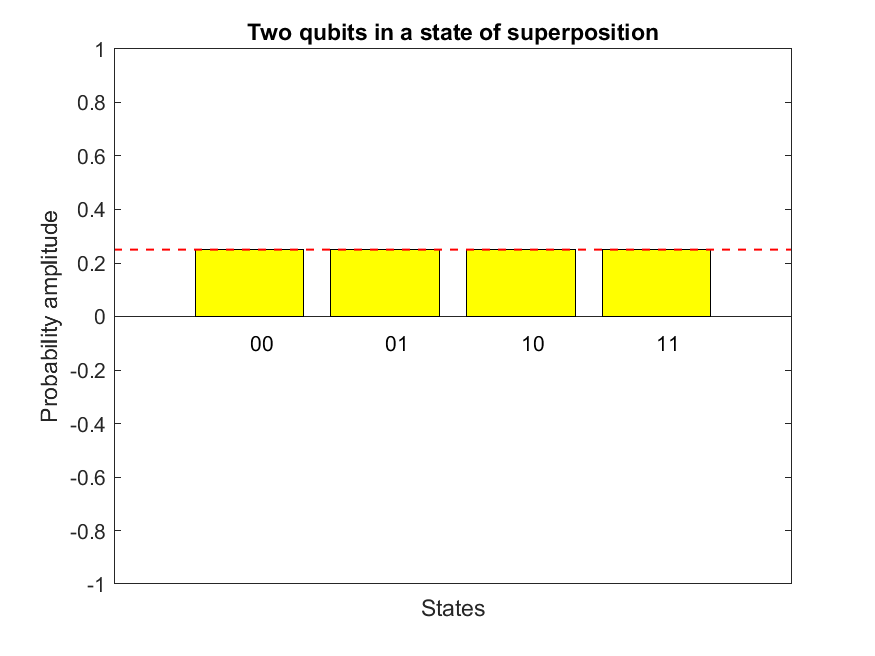
\includegraphics[width=9cm,height=10cm,keepaspectratio]{fig1.png}}
	\caption{Superposition of 2 qubits}
	\label{fig}
\end{figure}

\subsection{Oracle Function}
Grover’s algorithm hinges on the application of an oracle
function, often denoted as \textbf{"$ U_f $"}. This oracle acts to mark
the target state(s) by inverting their sign. For instance, if the
objective is to locate a specific item in a database, the oracle
would negate the amplitude corresponding to the target item.
In Fig. 2, it is graphically shown the oracle function flipping
the correct target.

\begin{figure}[htbp]
	\centerline{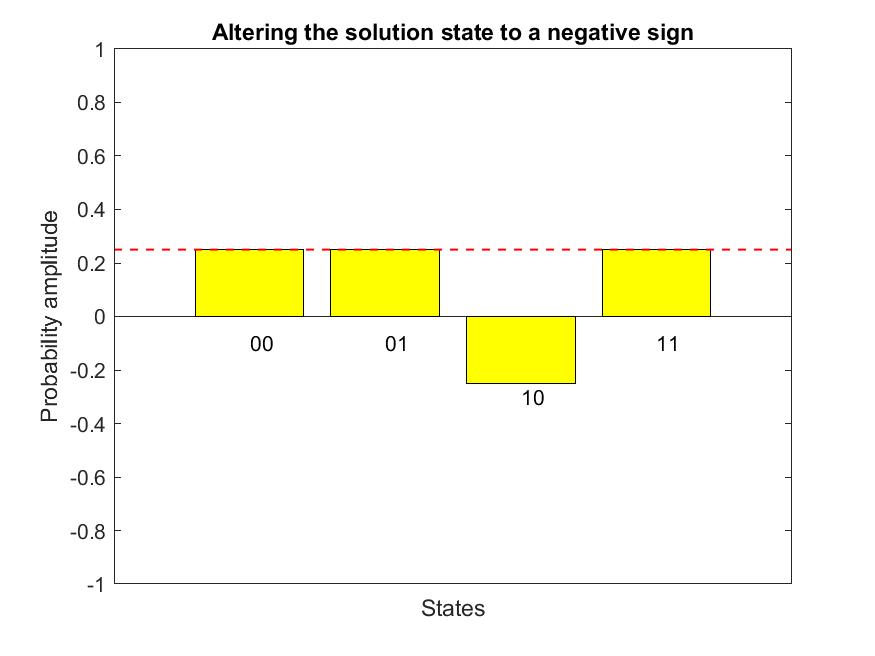
\includegraphics[width=9cm,height=10cm,keepaspectratio]{fig2.png}}
	\caption{Altering the sign of solution state(10)}
	\label{fig}
\end{figure}

\subsection{Amplitude Amplification}
The core of the Grover algorithm is the process of amplitude
amplification, which entails two central maneuvers:
\begin{itemize}
	\item \textbf{Inversion around the Mean}: During this stage, the amplitudes are mirrored around their average value, thus  boosting the amplitude of the desired state(s) while reducing the amplitudes of the non-desired states.
	\item \textbf{Grover diffusion operator}: In this step, the amplitudes
	      of the target state(s) are further augmented through the
	      application of a suite of quantum gates [10].

\end{itemize}
After acting of Grover diffusion operator, the final output will
have amplified magnitude as shown in Fig. 3.
\subsection{Reiteration}
Step. 2 and step. 3 are iterated approximately $ \sqrt{N} $ times
to maximize the likelihood of detecting the correct state. This
number of iterations ensures that the probability of identifying
the correct state approaches near certainty.

\begin{figure}[htbp]
	\centerline{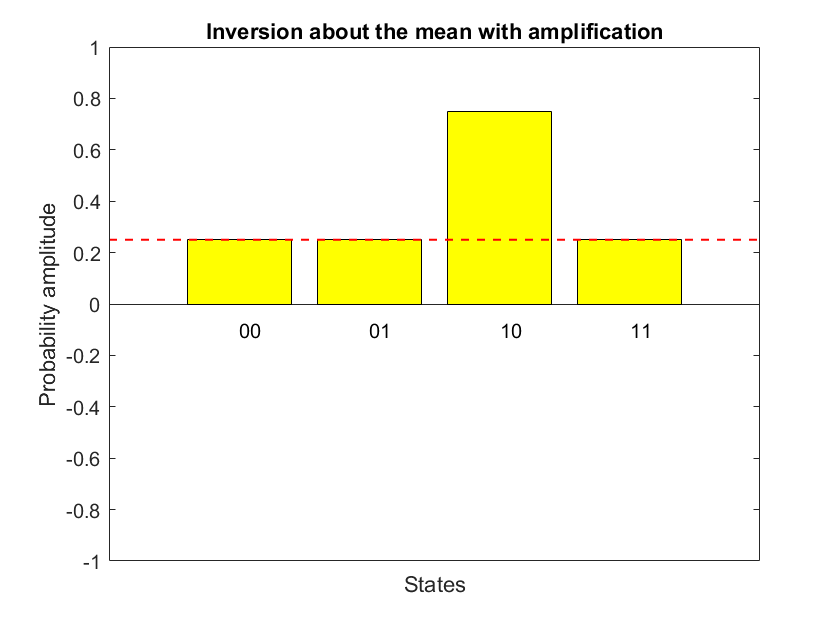
\includegraphics[width=9cm,height=10cm,keepaspectratio]{fig3.png}}
	\caption{Inversion about the mean with amplification.}
	\label{fig}
\end{figure}

\subsection{ Measurement}
Ultimately, the quantum state is subjected to measurement.
The target state is discerned with notably higher probability in comparison to the non-target state.

\section{Conclusion}
This study thoroughly investigated and modeled the Mott insulator V\textsubscript{2}O\textsubscript{3}, exploring its potential for ReRAM technology. The impact of various electrode configurations on device performance was carefully examined, identifying crucial areas for improvement crucial for successful integration. These results are pivotal for advancing the use of Mott materials in emerging memory technologies. The insights gained from this research are particularly valuable for developing a practical, physical model for future applications.




\begin{thebibliography}{00}

	\bibitem{b1} T. N. Theis and P. M. Solomon, "In Quest of the “Next Switch”: Prospects for Greatly Reduced Power Dissipation in a Successor to the Silicon Field-Effect Transistor," in Proceedings of the IEEE, vol. 98, no. 12, pp. 2005-2014, Dec. 2010.

	\bibitem{b2} Molas, G.; Nowak, E. "Advances in Emerging Memory Technologies: From Data Storage to Artificial Intelligence," Appl. Sci., vol. 11, no. 23, p. 1254, 2021.

	\bibitem{b3} J. H. de Boer, and E. J. W Verwey, "Semi-conductors with partially and with completely filled 3d-lattice bands," Proceedings of the Physical Society, vol. 49 (4S), pp. 4S, Aug.1937.

	\bibitem{b4} E. Janod, J. Tranchant, B. Corraze, M. Querré, P. Stoliar, M. Rozenberg, T. Cren et al. "Resistive switching in Mott insulators and correlated systems," Advanced Functional Materials, vol. 25, no. 40, pp. 6287-6305, Oct.2015.

	\bibitem{b5} J. Hubbard, "Electron correlations in narrow energy bands. II. The degenerate band case." Proceedings of the Royal Society of London. Series A. Mathematical and Physical Sciences, vol. 277, no. 1369, pp. 237-259, Jan.1964.

	\bibitem{b6} C. N. Berglund, "Thermal filaments in vanadium dioxide," in IEEE Transactions on Electron Devices, vol. 16, no. 5, pp. 432-437, May 1969.

	\bibitem{b7} A. Ronchi et al., "Light-Assisted Resistance Collapse in a V\textsubscript{2}O\textsubscript{3}-Based Mott-Insulator Device," Phys. Rev. Appl., vol. 15, no. 4, pp. 044023, Apr. 2021.

	\bibitem{b8} V. N. Andreev et al., "Thermal conductivity of VO\textsubscript{2}, V3O5, and V\textsubscript{2}O\textsubscript{3}," physica status solidi (a), vol. 48, no. 2, pp. K153-K156, 1978.

	\bibitem{b9} P. Stoliar et al., "Universal electric-field-driven resistive transition in narrow-gap Mott insulators," Adv. Mater., vol. 25, pp. 3222, 2013.

	\bibitem{b10} S. Guénon et al., "Electrical breakdown in a V\textsubscript{2}O\textsubscript{3} device at the insulator-to-metal transition," EPL (Europhysics Letters), vol. 101, pp. 57003, 2013.

	\bibitem{b11} P. Homm et al., "Collapse of the low temperature insulating state in Cr-doped V\textsubscript{2}O\textsubscript{3} thin films," Appl. Phys. Lett., vol. 107, pp. 111904, 2015.

	\bibitem{b12} Y. Kalcheim et al., "Non-thermal resistive switching in Mott insulator nanowires," Nat. Commun., vol. 11, pp. 2985, 2020.

	\bibitem{b13} M. M. Qazilbash et al., "Electrodynamics of the vanadium oxides VO\textsubscript{2} and V\textsubscript{2}O\textsubscript{3}," Phys. Rev. B, vol. 77, pp. 115121, 2008.

	\bibitem{b14} P. Paweł, J. Jamroz, and T. K. Pietrzak, “Observation of metal–insulator transition (mit) in vanadium oxides V\textsubscript{2}O\textsubscript{3} and VO\textsubscript{2} in xrd, dsc and dc experiments,” Crystals, 2023.

	\bibitem{b15} P. Homm, M. Menghini, J. W. Seo, S. Peters, and J. P. Locquet, “Room temperature Mott metal–insulator transition in V\textsubscript{2}O\textsubscript{3} compounds induced via strain-engineering,” APL Materials, vol. 9, no. 2, pp. 021116, Feb  2021.

	\bibitem{b16} F. Mazzola, S. K. Chaluvadi, V. Polewczyk, D. Mondal, J. Fujii, P. Rajak, M. Islam, R. Ciancio, L. Barba, M. Fabrizio, G. Rossi, P. Orgiani, and I. Vobornik, “Disentangling structural and electronic properties in V\textsubscript{2}O\textsubscript{3} thin films: A genuine non symmetry breaking mott transition,” Nano Letters, vol. 22, no. 14, pp. 5990–5996, 2022.

	\bibitem{b17} H. Kizuka et al., “Temperature dependence of thermal conductivity of VO\textsubscript{2} thin films across metal–insulator transition,” Japanese Journal of Applied Physics, vol. 98, no. 053201, 2015.

	\bibitem{b18} H. Y. Peng, L. Pu, J. C. Wu, D. Cha, J. H. Hong, W. N. Lin, Y. Y. Li, J. F. Ding, A. David, K. Li, and T. Wu, “Effects of electrode material and configuration on the characteristics of planar resistive switching devices,” APL Materials, vol. 1, no. 5, pp. 052106, Nov  2013.
\end{thebibliography}

\end{document}
